\documentclass[a4j, twocolumn, dvipdfmx]{jsarticle}

\usepackage[a4paper, left=2.0cm, right=2.0cm, top=2.0cm, bottom=2.0cm]{geometry}
\usepackage{amsmath}   % 数式用
\usepackage{amssymb}
\usepackage[dvipdfmx]{graphicx}
\usepackage{booktabs}  % \toprule, \midrule, \bottomrule 等の表罫線用
\usepackage{titlesec}  % 見出し調整
\usepackage{enumitem}  % 箇条書きの余白調整
\usepackage{array}
\usepackage{float}
\usepackage{flushend}  % 最終ページの左右コラムの高さをそろえる
\raggedbottom

% =========================================================
% 見出し設定（sotsuron_plan2.tex と統一）
% =========================================================
\titleformat{\section}[block]
  {\normalfont\large\bfseries}
  {\thesection}{0.7em}{}

\titleformat{\subsection}[block]
  {\normalfont\normalsize\bfseries}
  {\thesubsection}{0.7em}{}

\titleformat{\subsubsection}[block]
  {\normalfont\normalsize\bfseries}
  {\thesubsubsection}{0.7em}{}

\titleformat{\paragraph}[runin]
  {\normalfont\normalsize\bfseries}
  {\theparagraph}{0.5em}{}

\titlespacing*{\section}
  {0pt}{1.5ex plus 0.5ex minus 0.2ex}{0.8ex}
\titlespacing*{\subsection}
  {0pt}{1.2ex plus 0.4ex minus 0.2ex}{0.6ex}
\titlespacing*{\paragraph}
  {0pt}{1.0ex plus 0.3ex minus 0.1ex}{0.6em}

\setlist[itemize]{topsep=4pt, itemsep=2pt, parsep=0pt, leftmargin=*}
\setlist[enumerate]{topsep=4pt, itemsep=2pt, parsep=0pt, leftmargin=1.8em}

\newcolumntype{P}[1]{>{\raggedright\arraybackslash}p{#1}}

\title{
Federated Learningにおける悪性更新の検知可能性の評価 --- 実験結果報告\\
\large --- sotsuron\_plan2.tex 再スイープ（300実行）の結果 ---
}
\author{3CDA2216 笠原秀星}

\begin{document}

\maketitle

% =========================================================
\section{本報告の位置づけ}

本稿は, 研究計画書\cite{plan2}（\texttt{sotsuron\_plan2.tex}）の「再スイープ」の節で定めた実験（300実行, 出力先 \texttt{experiments\_detection\_v3}）の結果をまとめたものである. 以前の版の本稿は予備スイープ（27実行）の結果を報告していたが, その後データ分割方式・$\alpha$ の定義・ローカルエポック数・ALIEの $z$ の水準・試行数を改めたため, 数値は直接比較できない. 本稿はすべて再スイープの結果に置き換えた. 計画書に再スイープ前に記した3つの予測については, 当たったか外れたかをそのまま報告する（\S\ref{sec:predictions}）. 卒業論文の結果章・考察章の下書きとして用いることを想定する.

% =========================================================
\section{実験設定}

\begin{table}[H]
\centering
\caption{実験設定（再スイープ）}
\small
\begin{tabular}{@{}l@{\hspace{0.6em}}P{4.3cm}@{}}
\toprule
項目 & 値 \\
\midrule
データセット & MNIST \\
クライアント数 $n$ & 20（毎ラウンド全参加） \\
通信ラウンド数 & 50 \\
ローカルエポック数 & 2 \\
バッチサイズ / 学習率 & 32 / 0.01（SGD） \\
集約 & FedAvg \\
計算装置 & CPU \\
データ分割 & Hsuら\cite{hsu2019measuring}の $\mathrm{Dir}(\alpha\pi)$. 1台 $1{,}500$ 件（うち学習に $1{,}200$ 件） \\
Non-IID度 $\alpha$ & $1000\ (\approx\text{IID}),\ 5,\ 1$ \\
攻撃 & なし, 符号反転（A1）, ALIE（A2） \\
ALIEの $z$ & $0.385,\ 0.5,\ 0.75,\ 1,$ $1.25,\ 1.5,\ 2,\ 3$ \\
悪性割合 $f/n$ & $0.2$（$f=4$） \\
trial & $1$--$10$ \\
\bottomrule
\end{tabular}
\label{tab:setup}
\end{table}

\noindent
実行数は $3\,\alpha \times (\text{なし} + \text{A1} + \text{A2} \times 8\,z) \times 10\,\text{trial} = 300$ であり, 1実行あたり $50\,\text{ラウンド} \times 4\,\text{検知器} = 200$ 行, 全体で $60{,}000$ 行の検知指標を得た. 300実行すべてが50ラウンドまで完了している. 途中で失敗して回し直した実行があり, その途中までの行がログに残っている（検知指標のログで37件, 精度のログで42件）. 分析では条件ごとに最後の実行だけを用いた.

表\ref{tab:setup}の設定は, 実行時の設定記録（\texttt{run\_config.txt}）により, 分析に用いた300実行すべてで確認した. 計算装置は300実行すべてCPUであり, 実行期間は2026年10月12日から14日である. 悪性クライアントの選び方はtrialごとに固定されており, 同じtrialでは $\alpha$ と攻撃によらず同じ4台が悪性になる. クライアントごとの検知スコアとノルム（\texttt{detection\_updates.csv}）は, スコアから計算し直したAUCが検知指標のログと一致することを確認した. ただし, 1実行（$\alpha=1000$, ALIE $z=3$, trial 9）の第48ラウンドの行が欠けており, クライアント単位の集計ではこの実行のみ4ラウンド分となる. ラウンドごとのテスト精度（\texttt{results.csv}）は, 最終ラウンドの値が\texttt{summary.csv}と300実行すべてで一致することを確認した.

% =========================================================
\section{結果}

\subsection{グローバルモデルの精度}
\label{sec:accuracy}

表\ref{tab:accuracy}に50ラウンド時点のテスト精度を, 図\ref{fig:accuracy}に精度のラウンド推移を示す（いずれも10試行の平均$\pm$標準偏差）.

\begin{figure*}[t]
\centering
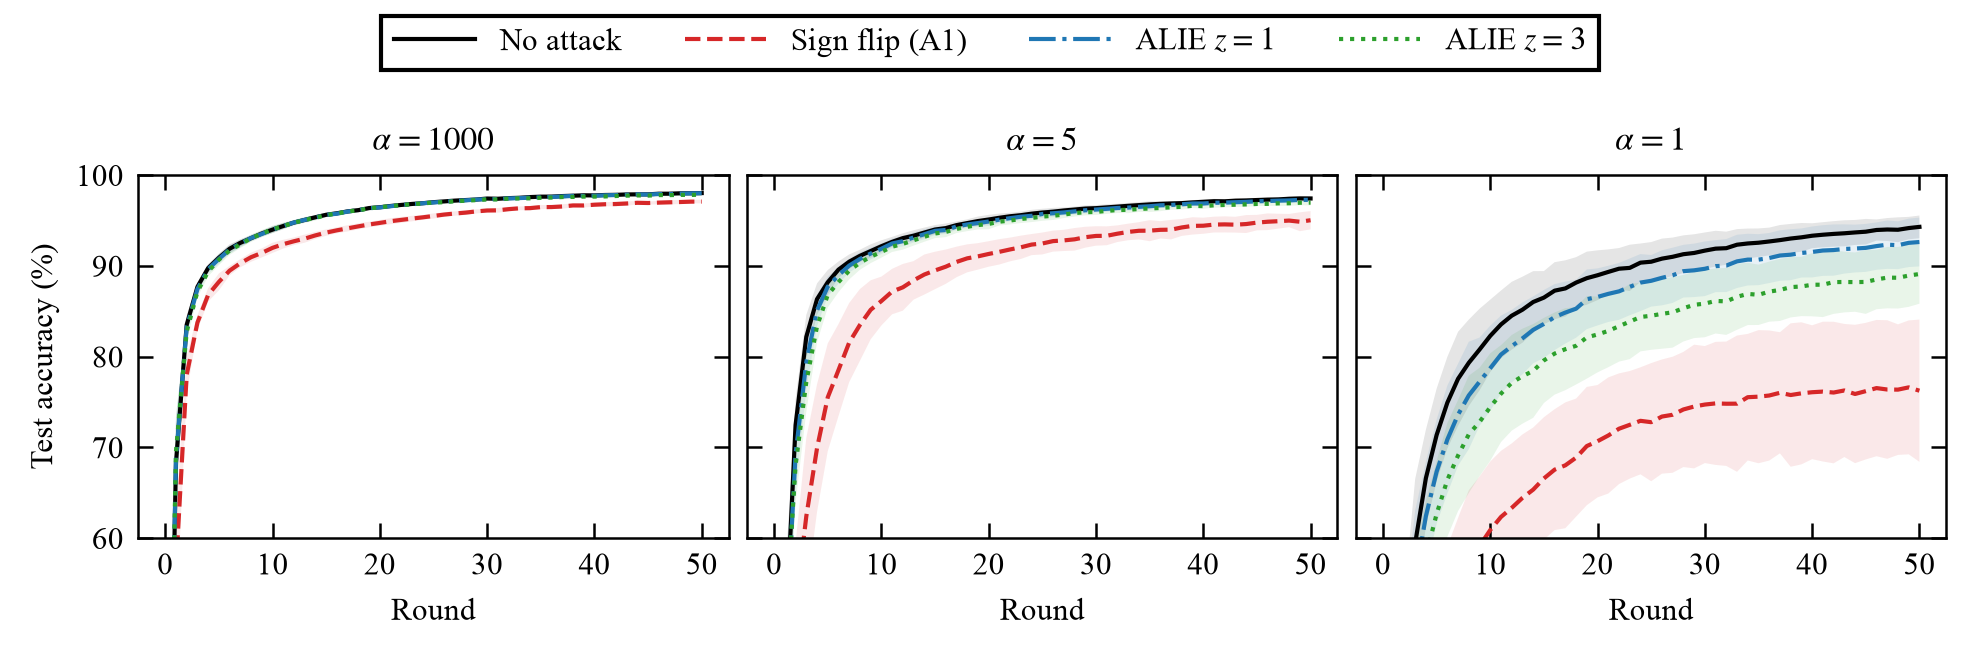
\includegraphics[width=0.8\textwidth]{experiments_detection_v3/_logs/analysis/accuracy_by_round.png}
\caption{テスト精度のラウンド推移（10試行の平均, 帯は$\pm$標準偏差）. ALIEは8通りの $z$ のうち $z=1$ と $z=3$ のみを示す. 縦軸は $60\%$ 以上を表示}
\label{fig:accuracy}
\end{figure*}

\begin{table}[H]
\centering
\caption{50ラウンド時点のテスト精度 [\%]（10試行の平均$\pm$標準偏差）}
\small
\tabcolsep=3pt
\begin{tabular}{@{}l@{\hspace{4pt}}ccc@{}}
\toprule
攻撃 & $\alpha=1000$ & $\alpha=5$ & $\alpha=1$ \\
\midrule
なし & $98.02 \pm 0.11$ & $97.43 \pm 0.24$ & $94.30 \pm 1.25$ \\
A1 符号反転 & $97.09 \pm 0.20$ & $95.03 \pm 1.01$ & $76.25 \pm 7.84$ \\
A2 $z=1$ & $98.01 \pm 0.10$ & $97.28 \pm 0.25$ & $92.63 \pm 2.69$ \\
A2 $z=2$ & $97.96 \pm 0.10$ & $97.19 \pm 0.26$ & $91.75 \pm 2.78$ \\
A2 $z=3$ & $97.86 \pm 0.11$ & $96.97 \pm 0.31$ & $89.11 \pm 3.28$ \\
\bottomrule
\end{tabular}
\label{tab:accuracy}
\end{table}

\noindent
符号反転は $\alpha=1$ で精度を約18ポイント下げ, 試行間のばらつきも大きい（最低 $63.2\%$）. ALIEは $\alpha \ge 5$ ではどの $z$ でも精度をほとんど下げない（攻撃なしとの差は最大0.5ポイント）. $\alpha=1$ では $z$ とともに精度が下がり, $z=3$ で攻撃なしより約5ポイント低い. $z \le 1.5$ の差は2ポイント以内である.

学習の収束を, 45ラウンドから50ラウンドまでの精度の上がり幅（10試行の平均）で確かめた. $\alpha=1000$ と $\alpha=5$ では, どの攻撃条件でも $0.11$--$0.26$ ポイントであり, 精度はほぼ頭打ちである. $\alpha=1$ では, 攻撃なしで $0.53$ ポイント, ALIEで $0.63$--$0.88$ ポイントとまだ上がり続けており, 50ラウンドでは収束していない. 計画書の事前確認（Flowerを介さない簡易な実行, 1試行）では $0.3$ ポイントであったが, 300実行では上がり幅がそれより大きかった. 一方, $\alpha=1$ の符号反転は $0.05$ ポイントであり, 約 $76\%$ で頭打ちになっている.

\subsection{ALIEに対する検知性能と $z$}
\label{sec:alie}

ALIEでは $\mathrm{push\_ratio}$ が構成上ほぼ $z$ に等しい（計画書の式）. 実測でも, 最終5ラウンド平均の $\mathrm{push\_ratio}$ はどの $\alpha$ でも $z$ の $1.00$--$1.02$ 倍であった. そこでALIEは $z$ を横軸に評価する. 図\ref{fig:auc-z}と表\ref{tab:alie-auc}に, 最終5ラウンド（46--50ラウンド）のAUCを, trialごとに平均してからtrial間の平均と標準偏差をとって示す.

\begin{figure*}[t]
\centering
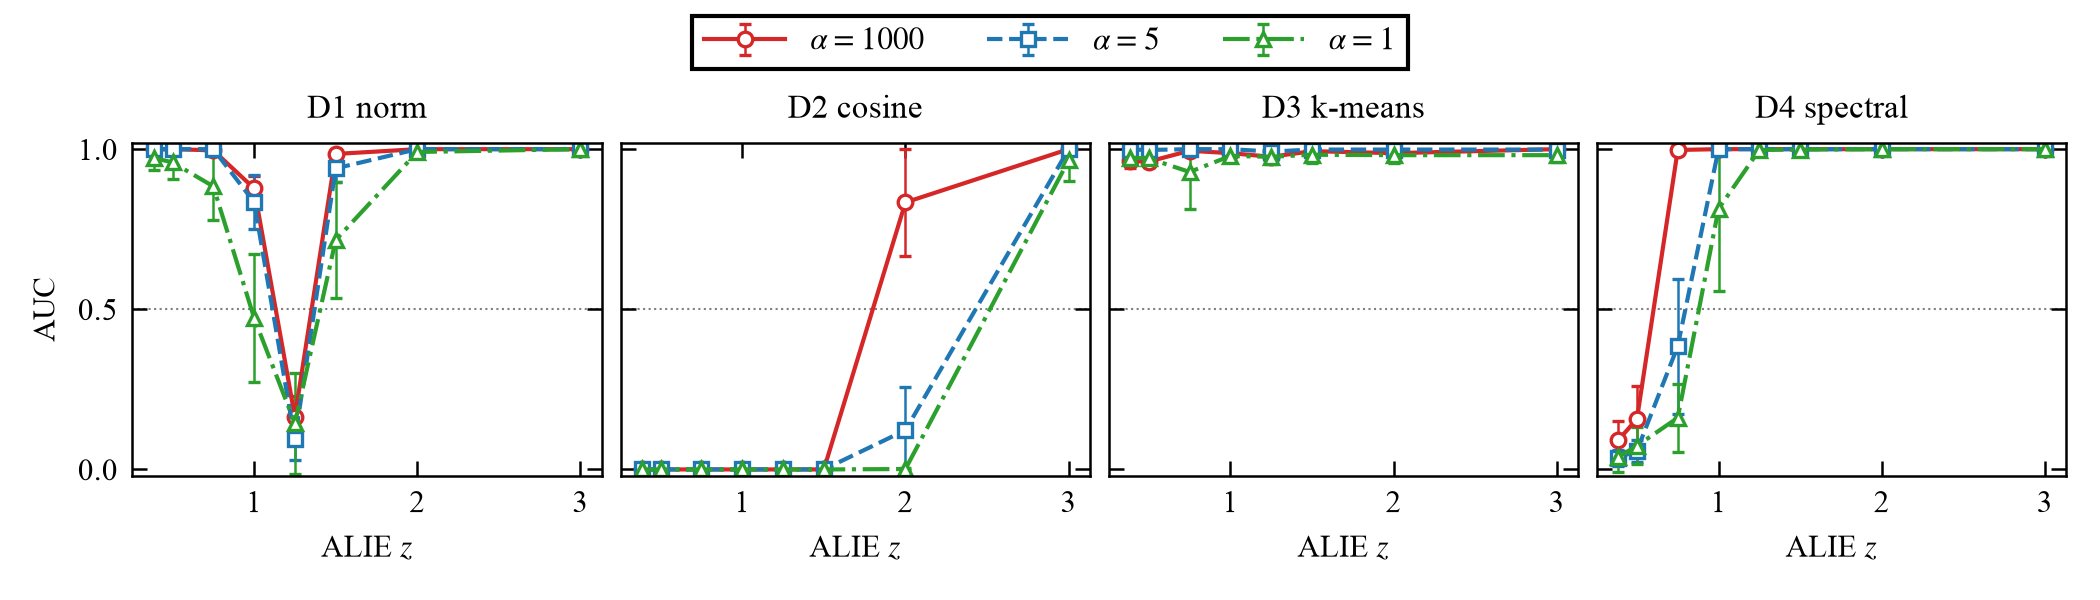
\includegraphics[width=\textwidth]{experiments_detection_v3/_logs/analysis/detection_auc_by_z.png}
\caption{ALIEの $z$ と最終5ラウンドのAUC. 点は10試行の平均, 棒は$\pm$標準偏差. 点線はAUC$=0.5$. AUCが $0$ に近いのは, 悪性のほうが一貫して正常らしいと判定されていることを表す}
\label{fig:auc-z}
\end{figure*}

\begin{table*}[t]
\centering
\caption{ALIEに対する最終5ラウンドのAUC（10試行の平均$\pm$標準偏差）. $z_{\max} \approx 0.385$ は原論文の式で $n=20,\ f=4$ から求めた値}
\footnotesize
\tabcolsep=4pt
\begin{tabular}{@{}c@{\hspace{6pt}}cccc@{\hspace{10pt}}cccc@{\hspace{10pt}}cccc@{}}
\toprule
 & \multicolumn{4}{c}{$\alpha=1000$} & \multicolumn{4}{c}{$\alpha=5$} & \multicolumn{4}{c}{$\alpha=1$} \\
$z$ & D1 & D2 & D3 & D4 & D1 & D2 & D3 & D4 & D1 & D2 & D3 & D4 \\
\midrule
0.385 & 1.00 & 0.00 & 0.96 & 0.09 & 1.00 & 0.00 & 1.00 & 0.04 & 0.97 & 0.00 & 0.97 & 0.04 \\
0.5   & 1.00 & 0.00 & 0.96 & 0.16$\pm$0.10 & 1.00 & 0.00 & 1.00 & 0.06 & 0.96 & 0.00 & 0.97 & 0.07 \\
0.75  & 1.00 & 0.00 & 0.99 & 1.00 & 1.00 & 0.00 & 1.00 & 0.39$\pm$0.21 & 0.88$\pm$0.10 & 0.00 & 0.93$\pm$0.12 & 0.16$\pm$0.11 \\
1     & 0.88 & 0.00 & 0.99 & 1.00 & 0.84 & 0.00 & 1.00 & 1.00 & 0.47$\pm$0.20 & 0.00 & 0.98 & 0.81$\pm$0.26 \\
1.25  & 0.16 & 0.00 & 0.98 & 1.00 & 0.09 & 0.00 & 0.99 & 1.00 & 0.14$\pm$0.16 & 0.00 & 0.98 & 1.00 \\
1.5   & 0.99 & 0.00 & 0.99 & 1.00 & 0.94 & 0.00 & 1.00 & 1.00 & 0.72$\pm$0.18 & 0.00 & 0.98 & 1.00 \\
2     & 1.00 & 0.83$\pm$0.17 & 0.99 & 1.00 & 1.00 & 0.12$\pm$0.13 & 1.00 & 1.00 & 0.99 & 0.00 & 0.98 & 1.00 \\
3     & 1.00 & 1.00 & 1.00 & 1.00 & 1.00 & 1.00 & 1.00 & 1.00 & 1.00 & 0.97 & 0.98 & 1.00 \\
\bottomrule
\end{tabular}
\par\smallskip
{\footnotesize 標準偏差は $0.10$ 以上のものだけを記した. 数値は\texttt{detection\_final\_auc\_table.csv}による.}
\label{tab:alie-auc}
\end{table*}

\noindent
検知器ごとの傾向は次のとおりである.
\begin{itemize}
  \item \textbf{D1（ノルム偏差）:} $z$ が小さいとほぼ完全に検知でき, $z$ を上げると低下し, $z=1.25$ で全 $\alpha$ とも最小（$0.09$--$0.16$）となったのち, $z \ge 1.5$ で再び上昇する. $\alpha=1$ では $z=0.75$--$1.5$ の範囲で他の $\alpha$ より低く, 試行間のばらつきも大きい. 最終5ラウンドの悪性更新のノルムの正常更新に対する比は, $z=0.385$ で $0.37$--$0.40$, $z=1$ で $0.84$--$0.85$, $z=1.25$ で $1.03$--$1.04$, $z=1.5$ で $1.21$--$1.23$ であり, D1が最小となる $z=1.25$ でノルムがほぼ揃っていた.
  \item \textbf{D2（コサイン距離）:} $z \le 1.5$ では全 $\alpha$ でAUCが $0.00$ であった. これは悪性更新が常に最も参照方向に近い（最も正常らしい）と判定されていることを意味し, 区別できていないのではなく逆向きに完全に分かれている. $z \le 1.5$ の全ラウンド平均のD2スコアは, 正常更新の $0.65$--$0.89$ に対して悪性更新は $0.21$--$0.23$ であった. $z=2$ で $\alpha$ による差が大きく（$0.83,\ 0.12,\ 0.00$）, $z=3$ で全 $\alpha$ とも検知に転じる.
  \item \textbf{D3（2クラスタリング）:} 全条件で $0.92$ 以上であり, $z$ にも $\alpha$ にもほとんど依存しない.
  \item \textbf{D4（スペクトル残差）:} $z$ が小さいと $0.04$--$0.16$ と逆向きに分かれ, ある $z$ を境に $1.0$ 近くへ急に切り替わる. 切り替わる $z$ は, $\alpha=1000$ で $0.5$--$0.75$ の間, $\alpha=5$ と $\alpha=1$ で $0.75$--$1$ の間にあり, $\alpha=1$ は $z=1$ でも $0.81$ にとどまる.
\end{itemize}

\subsection{符号反転に対する検知性能と $\mathrm{push\_ratio}$}
\label{sec:signflip}

\begin{table}[H]
\centering
\caption{符号反転に対する最終5ラウンドのAUC（10試行の平均$\pm$標準偏差）}
\footnotesize
\tabcolsep=3pt
\begin{tabular}{@{}c@{\hspace{4pt}}cccc@{}}
\toprule
$\alpha$ & D1 & D2 & D3 & D4 \\
\midrule
1000 & $0.97 \pm 0.07$ & $1.00 \pm 0.00$ & $1.00 \pm 0.00$ & $1.00 \pm 0.00$ \\
5    & $0.94 \pm 0.04$ & $1.00 \pm 0.00$ & $0.99 \pm 0.01$ & $0.97 \pm 0.04$ \\
1    & $0.88 \pm 0.08$ & $1.00 \pm 0.00$ & $0.98 \pm 0.03$ & $0.85 \pm 0.12$ \\
\bottomrule
\end{tabular}
\label{tab:sf-auc}
\end{table}

\begin{table}[H]
\centering
\caption{最終5ラウンド平均の正常更新の広がりと $\mathrm{push\_ratio}$}
\small
\begin{tabular}{@{}cccc@{}}
\toprule
 & \multicolumn{2}{c}{攻撃なし} & 符号反転 \\
$\alpha$ & $\mathrm{spread}$ & $\mathrm{pc1\_ratio}$ & $\mathrm{push\_ratio}$ \\
\midrule
1000 & $0.143$ & $0.086$ & $1.58$ \\
5    & $0.143$ & $0.122$ & $2.03$ \\
1    & $0.155$ & $0.193$ & $2.55$ \\
\bottomrule
\end{tabular}
\label{tab:spread}
\end{table}

\noindent
符号反転はD2・D3で全 $\alpha$ にわたりほぼ完全に検知でき, D1・D4は $\alpha$ が小さいほどやや低下する（D4: $1.00 \to 0.97 \to 0.85$）. 符号反転は更新の符号を反転するだけでノルムを変えないが, 悪性更新のノルムの正常更新に対する比は, 第1--5ラウンドの $1.00$--$1.15$ から最終5ラウンドの $1.30$（$\alpha=1000$）, $1.65$（$\alpha=5$）, $2.18$（$\alpha=1$）へ増大していた. D1が符号反転を検知できたのは, この学習過程を通じたノルムの変化によると考えられる. 一方, 正常更新の広がり $\mathrm{spread}$ は $\alpha=1000$ から $\alpha=1$ にかけて約8\%しか増えず, 符号反転の $\mathrm{push\_ratio}$ は $\alpha$ が小さいほど\textbf{大きく}なった（$1.58 \to 2.03 \to 2.55$）. 最終5ラウンドでの $\mathrm{push\_ratio}$ は全試行で $1.44$ 以上であり, $1$ を下回る領域は観測されなかった. 大きく変わったのは正常更新の広がり方の形であり, 第1主成分の寄与率 $\mathrm{pc1\_ratio}$ は $0.086 \to 0.122 \to 0.193$ と約2.2倍になった.

\begin{figure}[H]
\centering
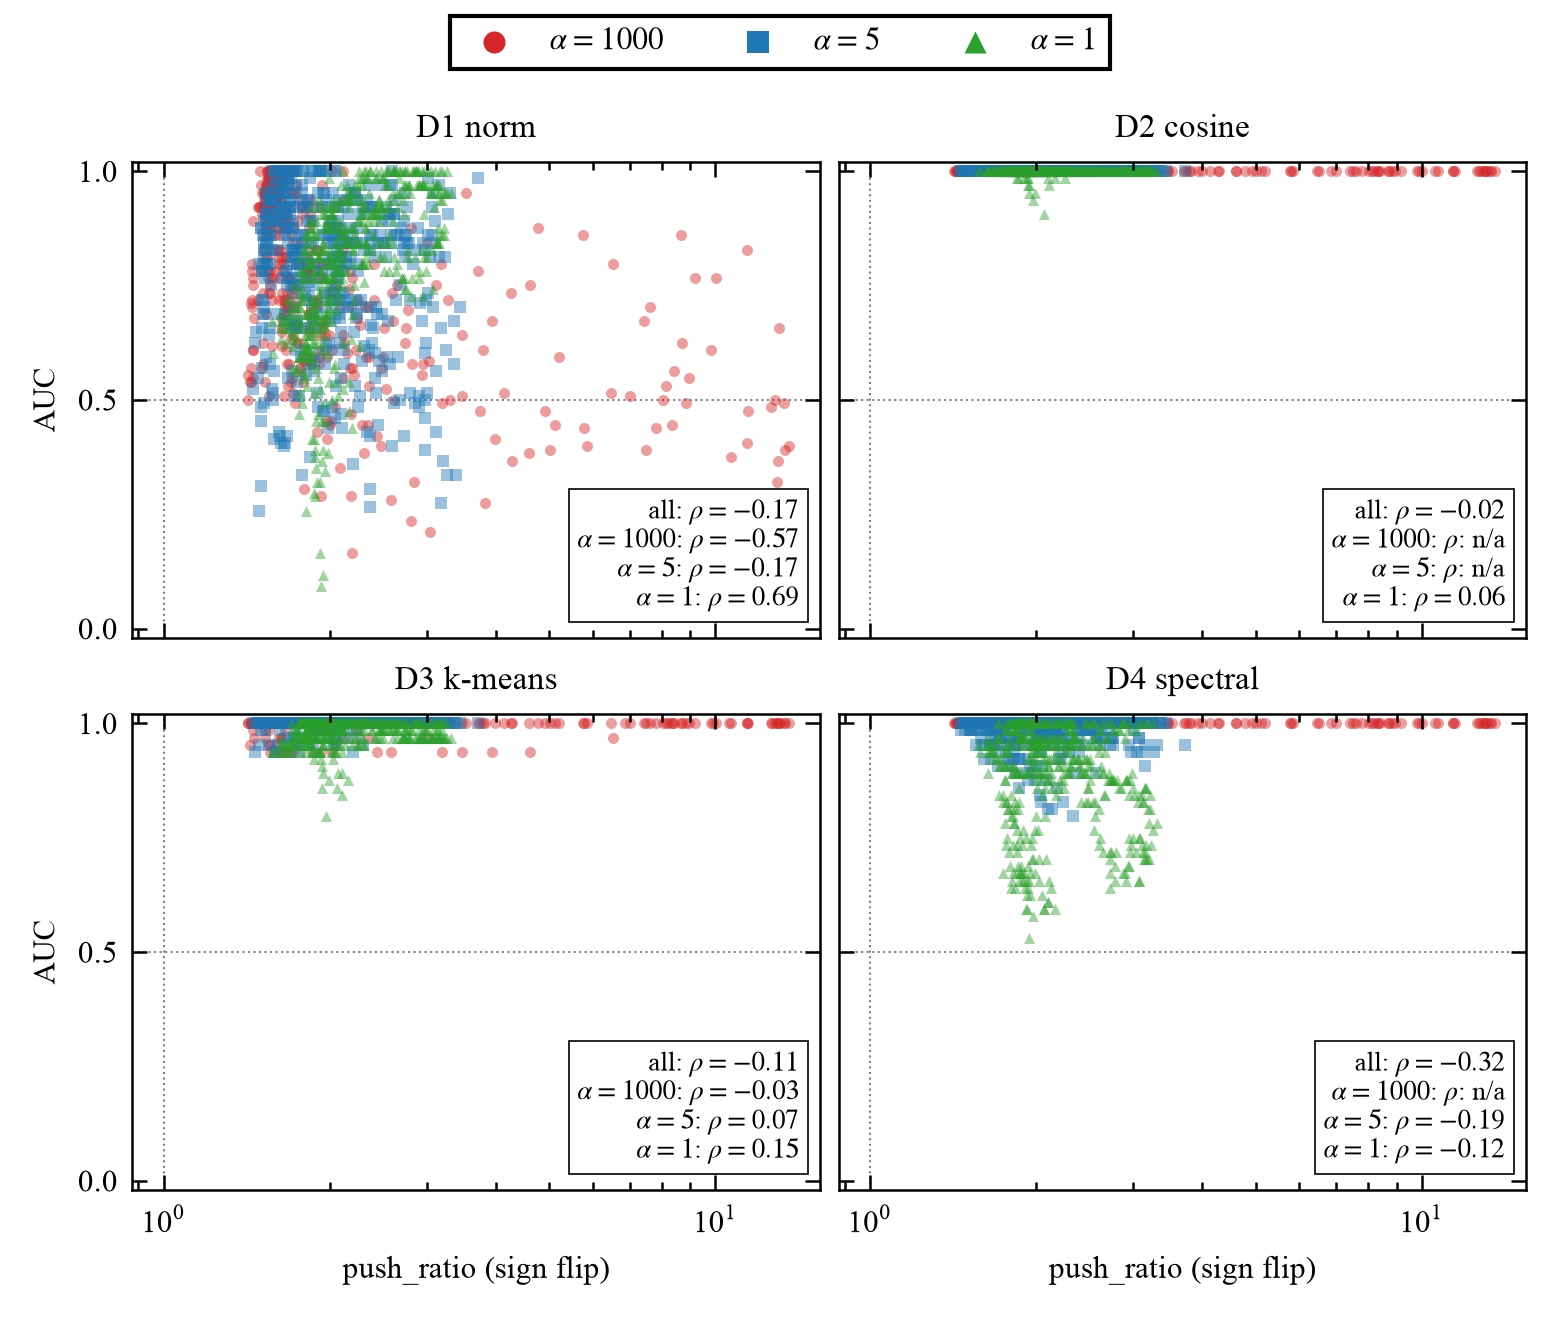
\includegraphics[width=\linewidth]{experiments_detection_v3/_logs/analysis/detection_pushratio_vs_auc.png}
\caption{符号反転における $\mathrm{push\_ratio}$（横軸, 対数）とAUC（縦軸）. 1点が1実行の1ラウンド（全ラウンド）. 右下は順位相関係数（全体と $\alpha$ ごと. n/a は AUC が一定で計算できないもの）}
\label{fig:pushratio}
\end{figure}

\begin{table}[H]
\centering
\caption{符号反転における $\mathrm{push\_ratio}$ とAUCの順位相関係数（全ラウンド, 1点=1実行の1ラウンド）}
\small
\begin{tabular}{@{}l@{\hspace{6pt}}rcccc@{}}
\toprule
$\alpha$ & 点数 & D1 & D2 & D3 & D4 \\
\midrule
全体 & 1{,}500 & $-0.17$ & $-0.02$ & $-0.11$ & $-0.32$ \\
1000 & 500 & $-0.57$ & n/a & $-0.03$ & n/a \\
5    & 500 & $-0.17$ & n/a & $0.07$ & $-0.19$ \\
1    & 500 & $0.69$ & $0.06$ & $0.15$ & $-0.12$ \\
\bottomrule
\end{tabular}
\label{tab:corr}
\end{table}

\noindent
$\mathrm{push\_ratio}$ とAUCの順位相関は, 全体でも $\alpha$ ごとでも弱いか負であった. 例外は $\alpha=1$ のD1（$0.69$）のみである. n/a は, その $\alpha$ でAUCがほぼ常に $1.0$ であり順位が付けられないことを表す.

\subsection{AUC対ラウンドの推移}

図\ref{fig:auc-round}に, 検知器（行）と攻撃（列）ごとのAUCのラウンド推移を示す. 最終5ラウンドの値だけでは見えない点として, 次の3つがある.
\begin{itemize}
  \item 符号反転に対するD1は, 序盤のAUCが $0.5$ 前後で, ラウンドとともに上がっていく.
  \item ALIEの $z=1.25$ に対するD1は, $\alpha=1000$ では序盤に高く, ラウンドとともに下がる.
  \item ALIEの $z=1.5$ に対するD2は, 最初の数ラウンドは高いが, 10ラウンド以内に $0$ へ下がる. $z=2$ でも $\alpha=5,\ 1$ では同様に下がる.
\end{itemize}

\begin{figure*}[t]
\centering
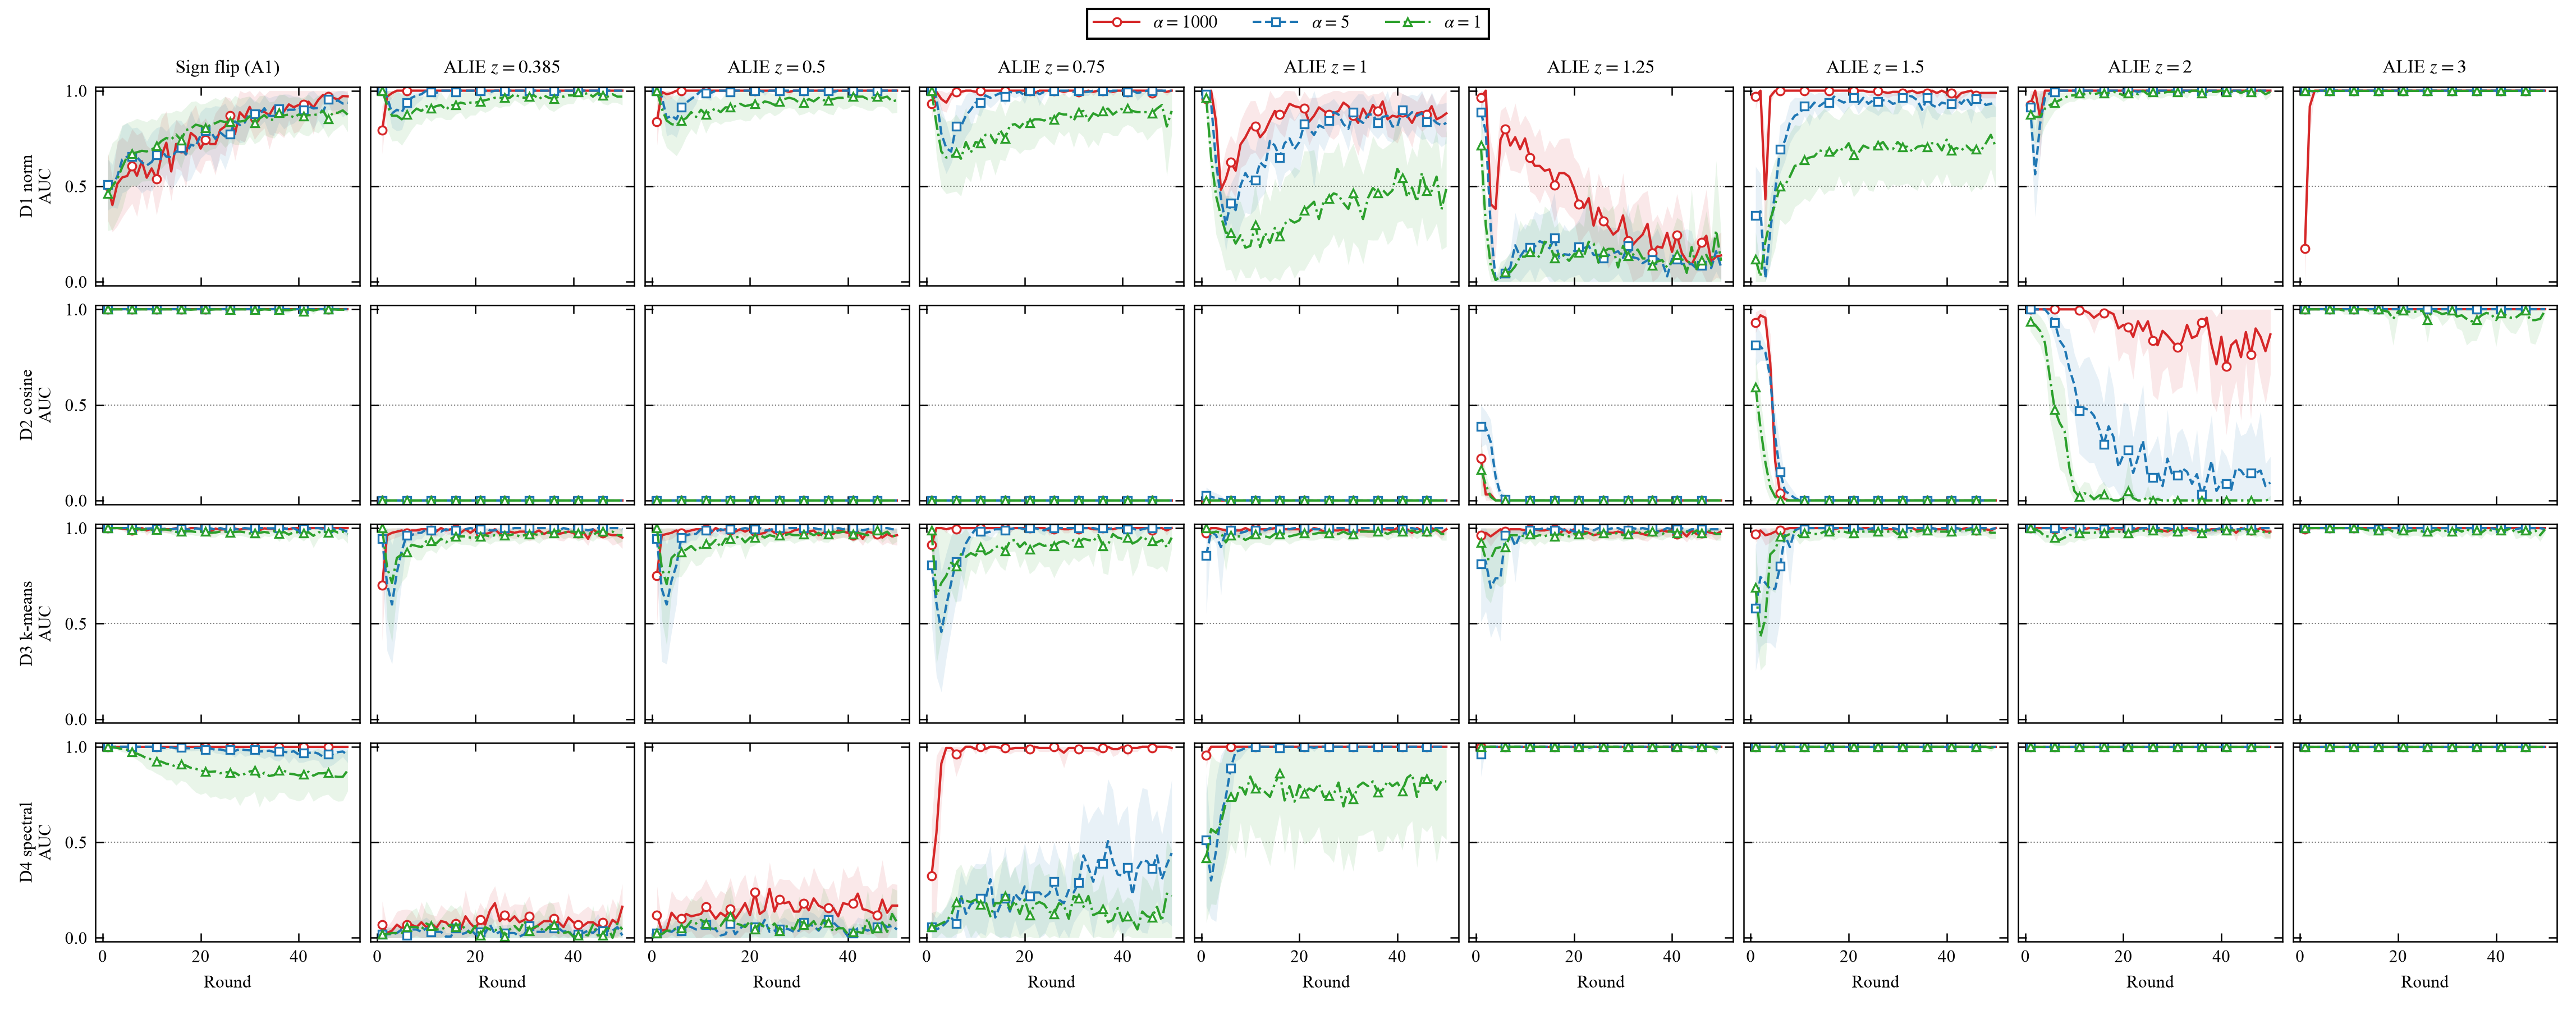
\includegraphics[width=\textwidth]{experiments_detection_v3/_logs/analysis/detection_auc_by_round.png}
\caption{AUC対ラウンド. 行は検知器D1--D4, 列は攻撃（ALIEの各 $z$ と符号反転）. 線はtrial平均, 帯は$\pm$標準偏差. 赤実線○: $\alpha=1000$, 青破線□: $\alpha=5$, 緑一点鎖線△: $\alpha=1$. 点線はAUC$=0.5$}
\label{fig:auc-round}
\end{figure*}

% =========================================================
\section{再スイープ前の予測の検証}
\label{sec:predictions}

計画書には, 再スイープの前に次の3つの予測を記していた.

\paragraph{予測1（D1は $z$ が $1$ をやや超える付近で最も低くなり, それより大きい $z$ で再び上昇する）．}
\textbf{当たった.} D1のAUCは全 $\alpha$ で $z=1.25$ が最小であり, $z=1.5$ 以上で再び上昇した（表\ref{tab:alie-auc}）. ALIEの悪性更新 $\mu - z\sigma$ のノルムは, $z$ が小さいと正常更新のノルムより小さく, $z$ を上げるにつれて大きくなる. 実際, 最終5ラウンドの悪性更新のノルムの正常更新に対する比は $z=0.385$ の $0.37$--$0.40$ から $z=3$ の $2.23$--$2.31$ まで増え, $z=1.25$ で $1.03$--$1.04$ とほぼ $1$ になった. ノルムが揃うこの点で, ノルムだけでは区別できなくなったと解釈できる.

\paragraph{予測2（D4は $\alpha=1$ でも $z$ を十分大きくすれば検知に転じ, 転じる $z$ はNon-IIDが強いほど大きい）．}
\textbf{当たった.} D4は $\alpha=1$ でも $z \ge 1.25$ でAUC $\ge 0.99$ となり, 検知に転じる $z$ は $\alpha=1000$ で最も小さく（$0.5$--$0.75$）, $\alpha=5$ と $\alpha=1$ ではそれより大きかった（$0.75$--$1$）. ただし $\alpha=5$ と $\alpha=1$ の差は, この $z$ の刻みでは区間として区別できず, $\alpha=1$ が $z=1$ で $0.81$ にとどまる点に表れるのみである.

\paragraph{予測3（$z \ge 2$ では, FedAvgのもとでもALIEがグローバルモデルの精度を低下させる可能性がある）．}
\textbf{一部当たった.} $\alpha=1$ では $z=2$ で約2.6ポイント, $z=3$ で約5.2ポイント, 攻撃なしより低下した. 一方 $\alpha \ge 5$ では, $z=3$ でも低下は0.5ポイント以内であった（表\ref{tab:accuracy}）.

% =========================================================
\section{考察}
\label{sec:discussion}

\subsection{中心仮説（A1）: 本設定では支持されなかった}

中心仮説は, Non-IIDが正常更新の広がりを増大させ, その結果 $\mathrm{push\_ratio}$ が下がって検知が難しくなる, というものであった. 再スイープの符号反転では, この連鎖のどちらの段階も観測されなかった. 第一に, データ数を揃えてラベル分布の偏りだけを変えた本設定では, $\mathrm{spread}$ は $\alpha$ によってほとんど変わらなかった（約8\%）. 第二に, 符号反転の $\mathrm{push\_ratio}$ は $\alpha$ が小さいほどむしろ大きくなり, $1$ を下回ることはなかった. 第三に, $\mathrm{push\_ratio}$ とAUCの順位相関は弱いか負であった.

一方で, D1とD4の検知性能は $\alpha$ が小さいほど低下しており, 「Non-IIDが検知を難しくする」こと自体は観測された. その低下は $\mathrm{push\_ratio}$ の変化では説明できない. 予備スイープで観測された $\mathrm{spread}$ の大きな増加は, データ数の偏りを含む分割方式と異なる学習設定のもとでのものであり, ラベル分布の偏りだけに起因するものではなかった可能性が高い. したがって, A1についての中心仮説は, 本研究の設定（データ数を揃えたラベル分布の偏り）では支持されなかった, と報告する.

\subsection{ALIE: $\mathrm{push\_ratio}$ では説明できない $\alpha$ の効果}

ALIEでは $\mathrm{push\_ratio}$ が $z$ でほぼ決まり, $\alpha$ によって変わらない. それにもかかわらず, 同じ $z$ で $\alpha$ によってAUCが大きく異なった. 最も顕著なのは $z=0.75$ のD4であり, $\mathrm{push\_ratio}$ がいずれも約 $0.75$ であるのに, AUCは $\alpha=1000,\ 5,\ 1$ の順に $1.00,\ 0.39,\ 0.16$ であった. これは, 検知性能が正常更新の広がりに対する相対距離だけでは決まらないことを示す.

この差と連動していたのは, 正常更新の広がり方の形である. 攻撃なし条件の $\mathrm{pc1\_ratio}$ は $\alpha=1000,\ 5,\ 1$ の順に $0.086,\ 0.122,\ 0.193$ であり, Non-IIDが強いほど正常更新が特定の方向へ細長く広がる. また, 悪性の押し出し方向と全更新の第1主成分の重なり $\mathrm{mal\_cos\_pc1\_all}$ は, D4のAUCとよく連動した（ALIEの24条件で順位相関 $0.92$, ラウンド単位で $0.85$）. D4は全更新の第1主成分への射影で判定するため, 悪性の押し出しが第1主成分になれば検知でき, 正常更新自体の細長い広がりが第1主成分を占めていれば検知できない. Non-IIDは正常更新の広がりの\textbf{大きさ}よりも\textbf{形}（異方性）を変え, それがD4の検知を妨げる, という解釈が考えられる.

ただし, この解釈は結果を見たあとに立てたものである. また, $\mathrm{mal\_cos\_pc1\_all}$ は正解ラベルを用いる量であり, D4の判定方法と直接結びついているため, D4が失敗する仕組みを言い換えている面がある. 独立な検証としては, 符号反転でも同じ関係が成り立つかを確かめる必要がある. 符号反転のD4でも, ラウンド単位で $\mathrm{mal\_cos\_pc1\_all}$ との順位相関は $0.75$ であった.

\subsection{検知器ごとの特徴}

\paragraph{D2の逆向きの分離．}
D2は $z \le 1.5$ のALIEに対して全 $\alpha$ でAUC $0.00$ であった. ALIEの悪性更新は正常更新の平均の近くに作られるため, 座標ごとの中央値を参照方向とするコサイン距離では, 悪性が最も正常らしく見える. AUCが低いことは「区別できない」ではなく「逆向きに完全に区別できる」ことであり, 外れ値を探す検知器にとって「典型的すぎる更新」が死角になることを示している. 類似度指標がこの種の攻撃に欺かれやすいことはWangら\cite{wang2023trust}が一般論として指摘しており, 本結果はそれがALIEに対して具体的に生じることを示す.

\paragraph{D3が常に高いこと．}
D3は全条件でAUC $0.92$ 以上であった. ALIEでは, 原論文のとおり悪性クライアント4台が同一のベクトルを送るため, 4点が互いに距離 $0$ の固まりになる. D3の高い性能はこの性質によるものである可能性があり, ALIEの摂動の巧妙さを見破っていることを意味するとは限らない. 悪性更新に小さな差をつけた場合の検証は, 本研究の範囲外である.

\subsection{精度への影響と検知の関係}

$\alpha \ge 5$ では, ALIEはどの $z$ でもモデルの精度をほとんど下げなかった. これは, 防御のない単純平均では攻撃の効果が薄まるという原論文\cite{baruch2019little}の報告と整合する. 一方, 符号反転は $\alpha=1$ で精度を約18ポイント下げたが, D2では全試行でほぼ完全に検知できていた. 本研究は検知結果を集約に用いていないが, 検知と除外を組み合わせれば精度の低下を防げる余地があることを示唆する.

% =========================================================
\section{妥当性への脅威と今後の課題}

\begin{itemize}
  \item \textbf{学習の収束:} $\alpha=1$ の学習は50ラウンドで収束しておらず, 45--50ラウンドでも精度が $0.5$--$0.9$ ポイント上がっている（\S\ref{sec:accuracy}）. $\alpha=1$ の最終5ラウンドの検知性能は, 学習が進みきる前の段階のものである. 検知性能のラウンド推移（図\ref{fig:auc-round}）を併せて示すことで補う.
  \item \textbf{ALIEの悪性更新が同一であること:} D3の高い性能の解釈に影響する. また, 同一の更新を調べるだけで検知できるという点は, この攻撃モデルの限界である.
  \item \textbf{事後の解釈:} \S\ref{sec:discussion}の「Non-IIDは広がりの形を変える」という解釈は結果を見てから立てたものであり, 別の条件で確かめる必要がある.
  \item \textbf{相関の点の独立性:} 表\ref{tab:corr}の順位相関は1実行の各ラウンドを1点として数えており, 同じ実行のラウンドどうしは独立ではない. 相関の大きさの目安として扱う.
  \item \textbf{回し直した実行:} 検知指標のログで37件, 精度のログで42件, 途中で失敗し回し直された実行の行が残っていた. 失敗の原因はログからは分からない.
  \item \textbf{規模と脅威モデル:} 20クライアント・MNIST・学習データの半分という小規模設定であり, full knowledge・悪性集合固定という前提のもとでの評価である.
  \item \textbf{発展課題（未実施）:} min-max／min-sum攻撃, 悪性割合の拡張, 検知と集約の統合評価は含まれない.
\end{itemize}

% =========================================================
\begin{thebibliography}{9}

\bibitem{plan2}
笠原秀星,
``Federated Learningにおける悪性更新の検知可能性の評価に関する研究計画書 --- データ分布の不均一性と攻撃のステルス性を軸とした更新ベクトルレベルの評価 ---,''
\texttt{sotsuron\_plan2.tex}, 2026.

\bibitem{baruch2019little}
Gilad Baruch, Moran Baruch, Yoav Goldberg,
``A Little Is Enough: Circumventing Defenses For Distributed Learning,''
Advances in Neural Information Processing Systems (NeurIPS), 2019.

\bibitem{hsu2019measuring}
Tzu-Ming Harry Hsu, Hang Qi, Matthew Brown,
``Measuring the Effects of Non-Identical Data Distribution for Federated Visual Classification,''
arXiv preprint arXiv:1909.06335, 2019.

\bibitem{shejwalkar2021manipulating}
Virat Shejwalkar, Amir Houmansadr,
``Manipulating the Byzantine: Optimizing Model Poisoning Attacks and Defenses for Federated Learning,''
Network and Distributed System Security Symposium (NDSS), 2021.

\bibitem{tran2018spectral}
Brandon Tran, Jerry Li, Aleksander Madry,
``Spectral Signatures in Backdoor Attacks,''
Advances in Neural Information Processing Systems (NeurIPS), 2018.

\bibitem{li2023experimental}
Shenghui Li, Edith C.-H. Ngai, Thiemo Voigt,
``An Experimental Study of Byzantine-Robust Aggregation Schemes in Federated Learning,''
arXiv preprint arXiv:2302.07173, 2023.

\bibitem{wang2023trust}
Zhilin Wang, Qin Hu, Xukai Zou,
``Can We Trust the Similarity Measurement in Federated Learning?,''
arXiv preprint arXiv:2311.03369, 2023.

\end{thebibliography}

\end{document}
